\part{Misura della costante di Rydberg}
\section{scopo e finalità}
	In questa parte di esperienza ci proponiamo dapprima di misurare la 
	risoluzione dello spettroscopio a reticolo in dotazione;
	e successivamente la misura della costante di Rydberg.
\section{strumentazione}
	La strumentazione impiegata 
	in questa sezione risulta analoga a quella impiega
	nella \sezione{sez:str_a}.
	Si è impiegato infatti uno spettrometro a reticolo.
	Tale spettroscopio si compone di:
	\begin{list}{$\cdot$}{}
		\item \textbf{una sorgente } ovvero una lampada al mercurio in fase di
		calibrazione, una lampada al sodio ,utilizzata per controllare la risoluzione dello strumento, e per effettare la misura di Rydberg
		una lampada al idrogeno.
		\item \textbf{due telescopi}, uno fisso	,per raccogliere la luce della 
		sorgente e inviarla sul reticolo, ed un telescopio di osservazione
		montato su di un piatto rotante e dotato di goniometro 
		(sensibilità di $1/120$ di grado),in grado di ruotare 
		rispetto al prisma.
		Il telescopio di raccolta  è munito di una fenditura regolabile
		attraverso la quale regolare l'ingresso della luce.
	
		Il telescopio di osservazione permette la regolazione del fuoco ed è 
		inoltre regolabile attraverso delle viti.
		\item \textbf{un prisma} che costituisce l'elemento dispersivo dello
		spettroscopio 
	\end{list}
	\bigskip
	si è inoltre impiegato una lente di ingrandimento per facilitare la lettura della scala del goniometro.

\bigskip


\begin{figure} [!h]
	\centering
	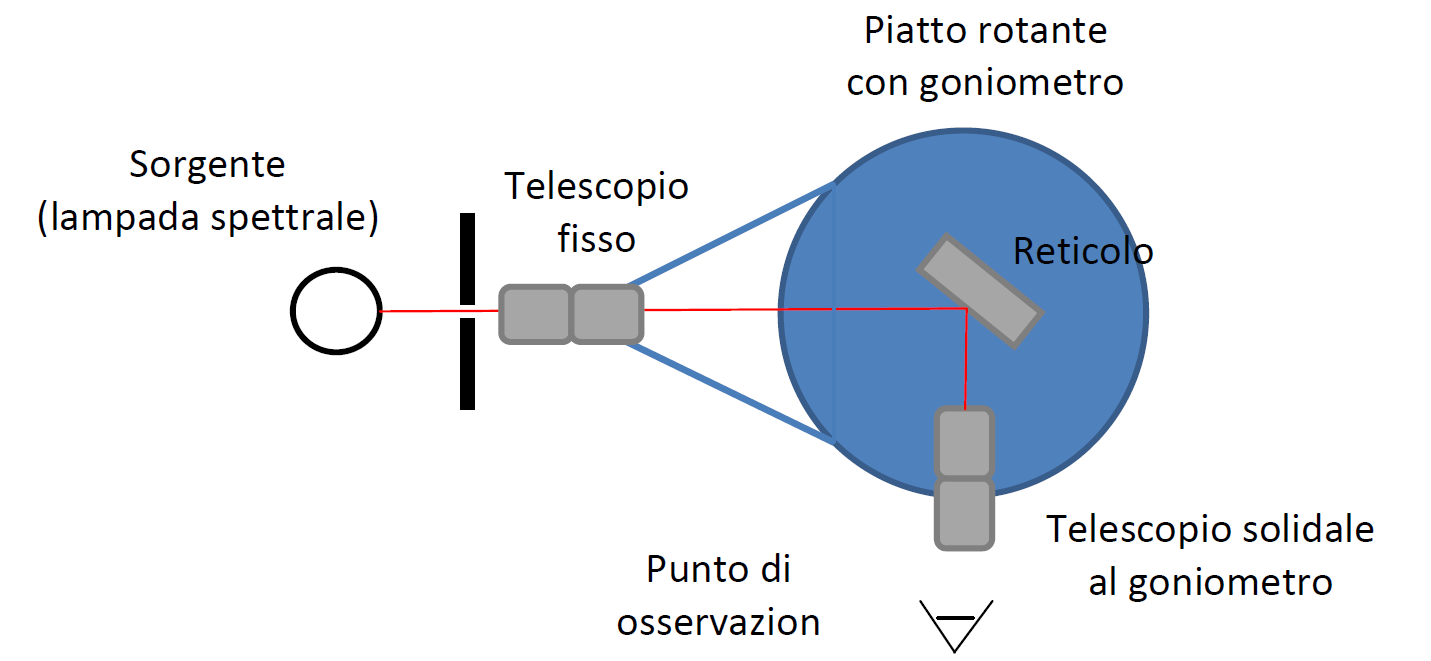
\includegraphics[width=0.9\textwidth]{./reticolo}
	\caption{Schema dell'apparato impiegato.}
	\label{fig:reticolo}
\end{figure}
Si riporta in \textbf{figura \ref{fig:reticolo} }uno schema dell'apparato
sperimentale impiegato. 